\documentclass[10pt]{article}
\usepackage[letterpaper,textwidth=5.5in,textheight=9in,centering]{geometry}
\usepackage{iftex}
\ifXeTeX\usepackage{fontspec}\setmainfont{texgyretermes}[Extension=.otf,UprightFont=*-regular,BoldFont=*-bold,ItalicFont=*-italic,BoldItalicFont=*-bolditalic]\else\usepackage{times}\fi
\usepackage[compact]{titlesec}
\titleformat*{\section}{\large\bfseries}
\titleformat*{\subsection}{\normalsize\bfseries}
\titlespacing*{\section}{0pt}{8pt}{3pt}
\titlespacing*{\subsection}{0pt}{6pt}{2pt}
\setlength{\textfloatsep}{8pt plus 2pt minus 2pt}
\setlength{\floatsep}{8pt plus 2pt minus 2pt}
\setlength{\abovecaptionskip}{3pt}
\renewcommand{\topfraction}{0.9}
\renewcommand{\textfraction}{0.1}
\setcounter{topnumber}{3}
\usepackage{amsmath,amssymb}
\usepackage{graphicx}
\usepackage{booktabs}
\usepackage{tabularx}
\usepackage{enumitem}
\usepackage[font=small,labelfont=bf]{caption}
\usepackage{xcolor}
\usepackage[hidelinks]{hyperref}
\graphicspath{{../figures/}}
\setlist{nosep,leftmargin=1.3em}
\setlength{\parindent}{0pt}
\setlength{\parskip}{5pt}
\newcommand{\todo}[1]{\textcolor{red}{[#1]}}

\title{\vspace{-0.6in}\rule{\linewidth}{3pt}\\[6pt]
\textbf{Probabilistic Graphical Models of U.S.\ Senate Roll-Call Voting}\\[2pt]\rule{\linewidth}{1pt}}
\author{\textbf{Conditionally Independent Caucus}\\
\todo{Name 1}, \todo{Name 2}, \todo{Name 3}, \todo{Name 4}, \todo{Name 5}}
\date{}

\makeatletter
\g@addto@macro\normalsize{\setlength\abovedisplayskip{4pt plus 1pt}\setlength\belowdisplayskip{4pt plus 1pt}%
\setlength\abovedisplayshortskip{2pt}\setlength\belowdisplayshortskip{2pt}}
\makeatother
\begin{document}
\maketitle
\vspace{-0.3in}

\begin{abstract}
\noindent The 2026 midterm elections are over, and a new Senate takes office in January. How predictable are
senators, and how much does the last Senate tell us about the next one? We study this with every roll-call vote of
the 117th and 118th Senates (Voteview, 100 senators each), using three graphical models that range from simple to
rich: a latent-class Naive Bayes model learned with EM, a Chow-Liu tree with exact belief propagation, and a sparse
Ising model learned by $\ell_1$-regularized pseudo-likelihood and queried with Gibbs sampling and mean-field. We
build everything from scratch and check it against brute-force enumeration. The simplest model gives the most
trustworthy probabilities: six hidden ``vote types'' predict hidden votes best (test NLL 0.136 per vote).
Mean-field is fast but overconfident when senators are tightly linked, EM copes with missing votes far better than
filling them in, and a model trained on one Senate predicts the next almost as well as one trained on it
directly.\footnote{Code and data: \url{https://github.com/TristoneLee/senate-pgm}.}
\end{abstract}

\section{Problem Description}
Every election reshuffles the Senate, yet a lot about how it votes stays the same: most senators vote with their
party, a few moderates cross over, and two senators from the same state often vote together. With the 2026 midterms
just finished and a new Senate arriving in January, it is a good moment to ask how much of this a probabilistic model
can actually capture.

We treat each senator's vote on a roll call as a yes/no random variable. These variables are clearly not
independent, and some are missing because senators skip votes. We ask three questions:
\begin{itemize}
\item \textbf{Q1 (prediction):} if we see how some senators voted, how well can we guess everyone else? Formally, we
want $P(X_i=\text{Yea}\mid\mathbf{x}_O)$ for every senator $i$ whose vote we have not seen.
\item \textbf{Q2 (structure):} what kind of dependence explains the votes best: a few hidden vote types, a tree of
pairwise links, or a web of pairwise links that may contain loops? And what does each model learn?
\item \textbf{Q3 (transfer):} does a model learned on one Senate still work on the next?
\end{itemize}
These questions use the core tools of the course: stating independence assumptions, learning with and without
missing data (MLE vs.\ EM), and choosing between exact and approximate inference. We care more about what each model
gets right and wrong than about squeezing out accuracy. Senate votes have been used the same way to test sparse
graphical models~\cite{banerjee2008}, and political scientists model them with spatial ``ideal point'' models such
as NOMINATE~\cite{poole1985} and its Bayesian counterparts~\cite{clinton2004}.

\section{Data Sourcing and Processing}
We use the Voteview roll-call database~\cite{voteview} for the 117th (2021--22) and 118th (2023--24) Senates:
individual votes, member metadata (party, state, NOMINATE scores) and roll-call metadata (date, vote question).
Each senator is a variable $X_i\in\{-1,+1\}$ (Nay/Yea) and each roll call is one sample.
\begin{itemize}
\item \textbf{Vote coding.} Cast codes 1--3 $\to$ Yea, 4--6 $\to$ Nay, 7--9 (present / not voting) and 0 (not
serving) $\to$ missing. Rows belonging to the Vice President's tie-breaking votes are dropped.
\item \textbf{Identity.} Senators are keyed by \texttt{bioguide\_id}, so a party switcher (e.g.\ Manchin, D$\to$I)
stays one variable instead of two half-missing ones.
\item \textbf{Filtering.} We drop near-unanimous roll calls (minority $<2.5\%$; 949$\to$906 and 691$\to$659),
which carry almost no information about dependencies, and senators present for under half of the roll calls,
leaving 100 senators per Congress.
\item \textbf{Splits.} Roll calls are split 80/20 by date into train and test (118th: 527/132). Hyper-parameters
are chosen on a \emph{validation} split (the last 20\% of training) and models are then refit on all training data,
so the test split is never used for any decision.
\item \textbf{Missing data.} The remaining missing rate is 3.9\% (117th) and 5.2\% (118th). We assume votes are
missing at random~\cite{rubin1976}; this is a simplification, because strategic absences exist.
\end{itemize}
Party, state and NOMINATE scores are \emph{never} model inputs; they are used only to interpret what was learned.
91 senators passed the filters in both Congresses and are used for the transfer experiment.
\textbf{Limitations:} a Congress has only $\sim$700--900 informative roll calls against $\binom{100}{2}=4950$
possible pairwise interactions, so the pairwise model needs strong regularization.

\section{Modeling and Inference}
All three models describe the same 100 yes/no variables, one per senator, for a single roll call; they differ only in
how votes may depend on each other. For each model we state the assumption, how it is learned, and how it answers
queries. Full update equations are in Appendix~\ref{app:alg}.

\subsection{M1: Latent-class Naive Bayes}
Each roll call has a hidden \emph{vote type} $Z\in\{1,\dots,K\}$ (for example ``a Democratic-backed party-line
vote''), and given the type, senators vote independently:
\begin{equation}
P(z,\mathbf x)=\pi_z\prod_{i=1}^{N}P(x_i\mid z),\qquad \theta_{iz}=P(X_i{=}{+}1\mid Z{=}z).
\end{equation}
\begin{itemize}
\item \textbf{Assumption.} All dependence between senators comes from the type of vote. A missing vote simply drops
out of the product, so it is marginalized exactly.
\item \textbf{Learning: EM}~\cite{dempster1977}. The E-step computes each roll call's posterior over types from its
observed votes, $\gamma_{mk}=P(Z^{(m)}{=}k\mid\mathbf x^{(m)}_O)$. The M-step re-estimates $\pi$ and $\theta$ as
$\gamma$-weighted vote frequencies with +1 (Laplace) pseudo-counts. We use 10 random restarts and check that the
objective never decreases.
\item \textbf{Inference: exact, $O(KN)$.} $P(X_i{=}{+}1\mid\mathbf x_O)=\sum_k\gamma_k\,\theta_{ik}$.
\end{itemize}

\subsection{M2: Chow-Liu tree Bayesian network}
M2 drops the hidden variable and links senators directly, but keeps only a tree of links so that inference stays
exact:
\begin{equation}
P(\mathbf x)=P(x_r)\prod_{i\ne r}P(x_i\mid x_{\mathrm{pa}(i)}).
\end{equation}
\begin{itemize}
\item \textbf{Assumption.} Given its parent's vote, a senator's vote is independent of all non-descendants in the
tree.
\item \textbf{Learning.} \emph{Structure:} the maximum-weight spanning tree on pairwise mutual information is the
maximum-likelihood tree~\cite{chowliu1968}. We estimate mutual information from the roll calls where both senators
voted and find the tree with Prim's algorithm. \emph{Parameters:} conditional probability tables by available-case
MLE (+1 Laplace), or by EM when votes are missing.
\item \textbf{Inference: exact sum-product belief propagation, $O(N)$.} One upward and one downward pass per roll
call give every senator's posterior and $\log P(\mathbf x_O)$; the same marginals form EM's E-step.
\end{itemize}

\subsection{M3: Sparse Ising model (pairwise Markov network)}
A tree cannot contain loops, such as three moderates who all vote together. M3 allows any sparse set of pairwise
links:
\begin{equation}
P(\mathbf x)=\frac{1}{Z(\theta,W)}\exp\Big(\sum_i\theta_ix_i+\sum_{i<j}W_{ij}x_ix_j\Big),\qquad x_i\in\{-1,+1\}.
\end{equation}
Here $\theta_i$ is senator $i$'s baseline lean toward Yea, and $W_{ij}>0$ ($<0$) means $i$ and $j$ tend to agree
(disagree).
\begin{itemize}
\item \textbf{Assumption.} Given its neighbors' votes, a senator's vote is independent of everyone else; only
pairwise interactions exist.
\item \textbf{Learning: $\ell_1$-penalized pseudo-likelihood}~\cite{besag1975,ravikumar2010}. The normalizer
$Z(\theta,W)$ sums over $2^{100}$ vote patterns, so exact maximum likelihood is impossible. Instead we fit each
senator's vote given everyone else's, $P(x_i\mid\mathbf x_{-i})=\sigma\big(2x_i(\theta_i+\sum_jW_{ij}x_j)\big)$,
with a penalty $\lambda\sum_{i<j}|W_{ij}|$ that sets most couplings to zero. The objective is convex, and we solve it
with FISTA~\cite{beck2009}. Missing votes enter as $x_j=0$.
\item \textbf{Inference: approximate.} With the observed votes fixed, we use \emph{Gibbs
sampling}~\cite{geman1984} (4 chains with burn-in) and \emph{naive mean-field}~\cite{wainwright2008}
($\mu_i\leftarrow\tanh(\theta_i+\sum_jW_{ij}\mu_j)$). For a 16-senator model we also enumerate all $2^{16}$ states
exactly, which serves as ground truth in E1.
\end{itemize}

\subsection{Implementation and verification}
Everything is implemented in Python with NumPy/SciPy. Before touching real data, we checked every routine against
brute force on random 6-variable models: M1 inference, M2's marginals and $\log P(\mathbf x_O)$, and Ising
enumeration agree to $<10^{-14}$, and Gibbs (3000 sweeps) to $1.4\times10^{-3}$. On synthetic data with 30\% of the
votes missing, EM recovers M1's parameters to within 0.05, and Chow-Liu recovers 26 of 29 edges of a known tree
(Appendix, Table~\ref{tab:checks}).

\section{Results and Discussion}
We present results in three layers: \S4.1 states what each experiment shows statistically, \S4.2 compares the
models' strengths and weaknesses, and \S4.3 collects what the models reveal about the Senate itself.
\textbf{Hyper-parameters} were chosen on the validation split only (Appendix, Fig.~\ref{fig:selection}): $K=6$
coalition types (validation log-likelihood is flat beyond $K=5$), and $\lambda=0.01$ / $0.02$ for M3 (117th / 118th),
selected by NLL on the same 20\%-reveal task used in E3. All learners converge monotonically (EM in 7--22
iterations, FISTA in 389; Appendix, Fig.~\ref{fig:conv}).

\subsection{Statistical findings}

\textbf{E1: How accurate is approximate inference?} We fit a 16-senator Ising model (8 D, 8 R; $\lambda=0.2$,
max $|W_{ij}|=0.74$), clamp 4 senators on each of 132 test roll calls, query the other 12, and compare against exact
enumeration of all $2^{16}$ states while scaling the couplings $W\to\beta W$, $\beta\in[0.1,2]$ (Fig.~\ref{fig:e1}).
\begin{itemize}
\item \emph{Mean-field is fast but biased, and overconfident when couplings are strong.} Its error is 0.033 at
$\beta=1$, about 8$\times$ that of Gibbs. The absolute error falls again at $\beta=2$ (0.018) only because
marginals saturate near 0 or 1; the KL divergence keeps rising (0.0007 at $\beta=0.5$, 0.010 at $\beta=1$,
0.015--0.020 for $\beta\ge1.5$).
\item \emph{Gibbs converges at the Monte Carlo rate.} At $\beta=1$ the error drops from 0.021 (10 sweeps) to 0.002
(1000 sweeps); 300 sweeps keep it $\le0.004$ for every $\beta$, at 10--70$\times$ the cost of mean-field.
\item \emph{Exact inference only works for tiny models}: $2^{16}$ states take under 0.1\,s, $2^{100}$ is impossible.
\end{itemize}

\begin{figure}[t]
\centering
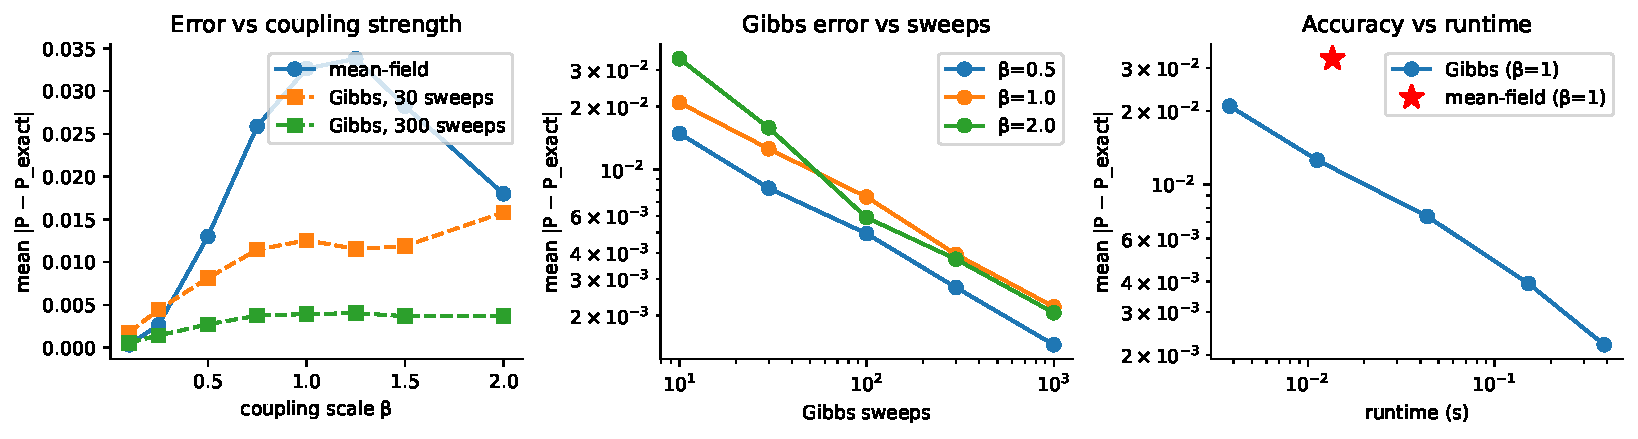
\includegraphics[width=0.85\linewidth]{E1_inference.pdf}
\vspace{-6pt}
\caption{E1. Mean absolute error of approximate marginals against exact enumeration (16-senator Ising model).}
\label{fig:e1}
\end{figure}

\textbf{E2: How should missing votes be handled?} We hide 10/30/50\% of the 118th training votes (3 masks each)
and measure held-out log-likelihood and accuracy on the hidden votes (Fig.~\ref{fig:e2}).
\begin{itemize}
\item \emph{Marginalize, do not impute.} M1 with EM barely changes (LL $-0.143\to-0.150$, accuracy $\approx0.94$
throughout). Filling gaps with each senator's majority vote collapses at 50\% (LL $-0.184$, accuracy 0.78), because
the fake votes erase the minority vote types.
\item \emph{Under random masking, EM and available-case counting agree} for M2 (differences $<0.002$): both are
consistent, and EM only adds efficiency.
\item \emph{Stochastic EM gives M3 a small gain that grows with missingness} (0.948 vs.\ 0.940 at 50\%).
\end{itemize}

\begin{figure}[t]
\centering
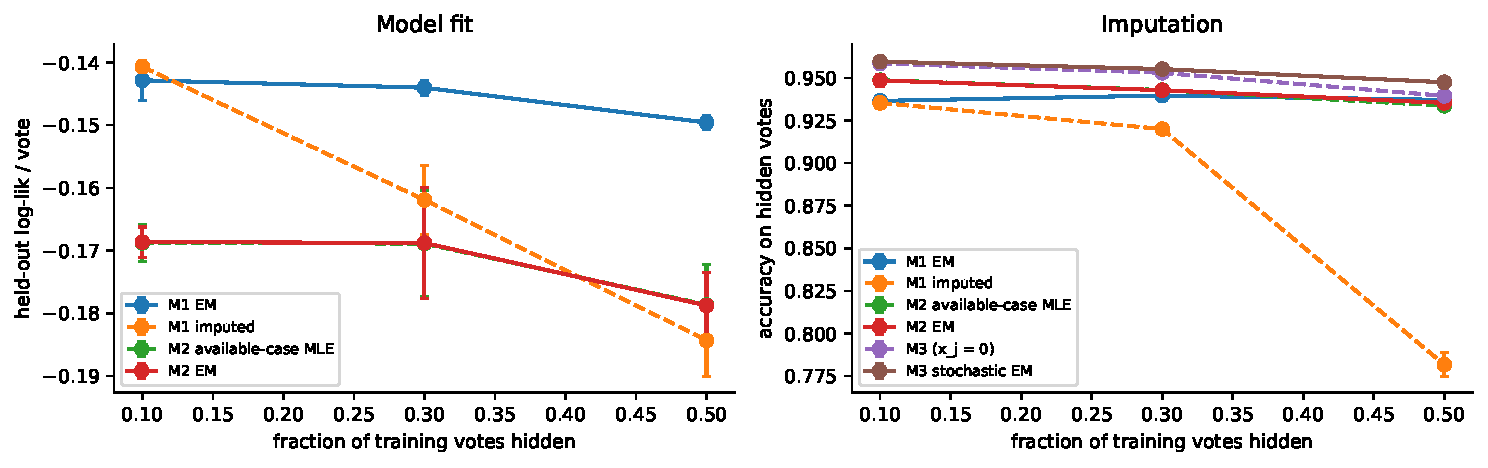
\includegraphics[width=0.8\linewidth]{E2_missing.pdf}
\caption{E2. Left: held-out log-likelihood per vote (M1, M2). Right: accuracy on the hidden training votes. Mean
$\pm$ std over 3 masks.}
\label{fig:e2}
\end{figure}

\textbf{E3: How well can we predict hidden votes?} On each test roll call we reveal 20\% of the observed votes and
predict the rest (5 reveals; Table~\ref{tab:e3}). Two references: each senator's training Yea rate (no dependencies),
and ``vote with your party's revealed majority'', which uses party labels the models never see.
\begin{itemize}
\item \emph{All three models capture the dependencies:} they beat the per-senator baseline by a wide margin and
match or beat the party baseline without knowing parties.
\item \emph{Accuracy ties, calibration does not.} Accuracies are within 0.005 of each other, but M1 has the lowest
NLL in both Congresses (0.170 / 0.136). M3 with Gibbs has the best 118th accuracy (0.949).
\item \emph{Errors concentrate on cross-cutting votes}: 0.97 accuracy on the 112 party-line roll calls vs.\
0.83--0.84 on the 20 cross-cutting ones.
\item \emph{The selection criterion mattered more than the sampler} (Appendix, Table~\ref{tab:diag}): 10$\times$
more Gibbs sweeps change NLL by $<0.004$, while choosing $\lambda$ by pseudo-likelihood ($\lambda=0.05$) drops M3 to
0.912 / 0.233 in the 117th.
\end{itemize}

\begin{table}[t]
\centering\small
\caption{E3. Prediction of the 80\% hidden votes on test roll calls (mean over 5 reveals; std $\le0.003$ accuracy,
$\le0.015$ NLL).}
\label{tab:e3}
\begin{tabular}{lcccccc}
\toprule
& \multicolumn{3}{c}{117th Senate} & \multicolumn{3}{c}{118th Senate}\\
\cmidrule(lr){2-4}\cmidrule(lr){5-7}
Model & Acc & NLL & AUC & Acc & NLL & AUC\\
\midrule
Per-senator Yea rate & 0.655 & 0.654 & 0.661 & 0.873 & 0.445 & 0.900\\
Party majority (uses labels) & 0.911 & 0.235 & 0.966 & 0.949 & 0.169 & 0.982\\
M1 latent class (EM) & \textbf{0.934} & \textbf{0.170} & \textbf{0.981} & 0.945 & \textbf{0.136} & \textbf{0.989}\\
M2 Chow-Liu tree (BP) & 0.930 & 0.200 & 0.974 & 0.947 & 0.165 & 0.980\\
M3 Ising, Gibbs & 0.930 & 0.194 & 0.979 & \textbf{0.949} & 0.152 & 0.986\\
M3 Ising, mean-field & 0.929 & 0.242 & 0.976 & 0.946 & 0.187 & 0.981\\
\bottomrule
\end{tabular}
\end{table}

\textbf{E4: Does a model carry over to the next Senate?} We use the 91 senators who served in both Congresses
(Fig.~\ref{fig:e4}).
\begin{itemize}
\item \emph{Direct transfer is almost free.} Trained only on the 117th, the models predict the 118th test votes about
as well as models trained on the 118th (NLL: M1 0.143 vs.\ 0.140, M2 0.167 vs.\ 0.172, M3 0.175 vs.\ 0.200).
Keeping M1's 117th $\theta$ and refitting only the mix $\pi$ gives 0.141.
\item \emph{A prior from the previous Senate replaces most of the data.} With 10 roll calls of the 118th, M1 scores
0.280 without a prior and 0.144 with the $s{=}100$ prior; without it, 200--527 roll calls are needed to get there.
Prior plus all data is the best model overall (0.136).
\item \emph{The prior must be strong enough}: with $s{=}10$, EM drifts away from the good start on 25--100 roll calls.
\end{itemize}

\begin{figure}[t]
\centering
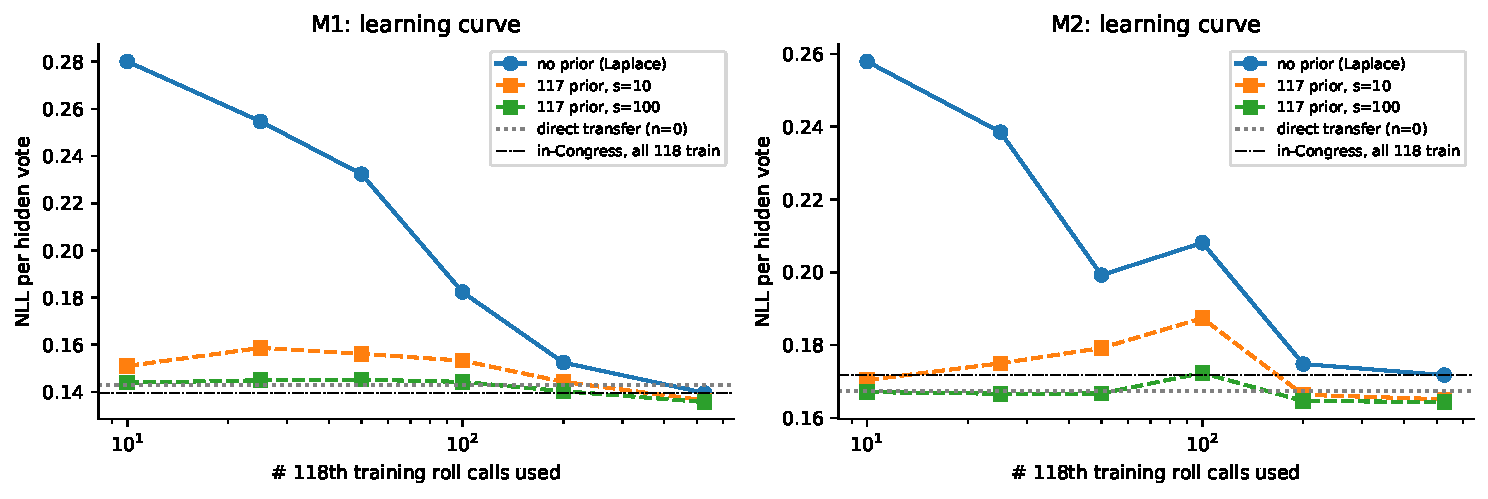
\includegraphics[width=0.8\linewidth]{E4_transfer_curve.pdf}
\caption{E4. Prediction NLL on 118th test roll calls vs.\ number of 118th training roll calls, with and without the
117th-Senate prior.}
\label{fig:e4}
\end{figure}

\subsection{Model strengths and weaknesses}
Table~\ref{tab:models} summarizes when each model is the right tool. The key structural point: a single hidden vote
type influences every senator at once, and once it is summed out, all 100 votes depend on each other. M1 represents
this directly with one variable; a sparse pairwise model can only approximate it with many couplings, which is why
M3 matches M1's accuracy but not its calibration.

\begin{table}[t]
\centering\small
\caption{Strengths and weaknesses of the three models, with the evidence from our experiments.}
\label{tab:models}
\begin{tabularx}{\linewidth}{@{}l>{\raggedright\arraybackslash}X>{\raggedright\arraybackslash}X>{\raggedright\arraybackslash}X@{}}
\toprule
& \textbf{M1 latent class} & \textbf{M2 Chow-Liu tree} & \textbf{M3 sparse Ising}\\
\midrule
Strengths & best calibration (lowest NLL); readable vote types; robust to missing data; transfers with a prior & exact $O(N)$ inference; cheapest; quick overview of the party structure & finds specific alliances; best on the Collins--Murkowski pair (0.65 vs.\ 0.50); top 118th accuracy\\
Weaknesses & fails on votes unlike any of its $K$ types; no senator-to-senator links & only 6 cross-party edges, so evidence passes between parties through very few links & approximate inference only; mean-field overconfident; $\lambda$ must be tuned to the task\\
Use it for & default predictor; missing data; new Senates & fast exact queries & studying who votes with whom\\
\bottomrule
\end{tabularx}
\end{table}

\begin{figure}[t]
\centering
\begin{minipage}[c]{0.44\linewidth}\centering
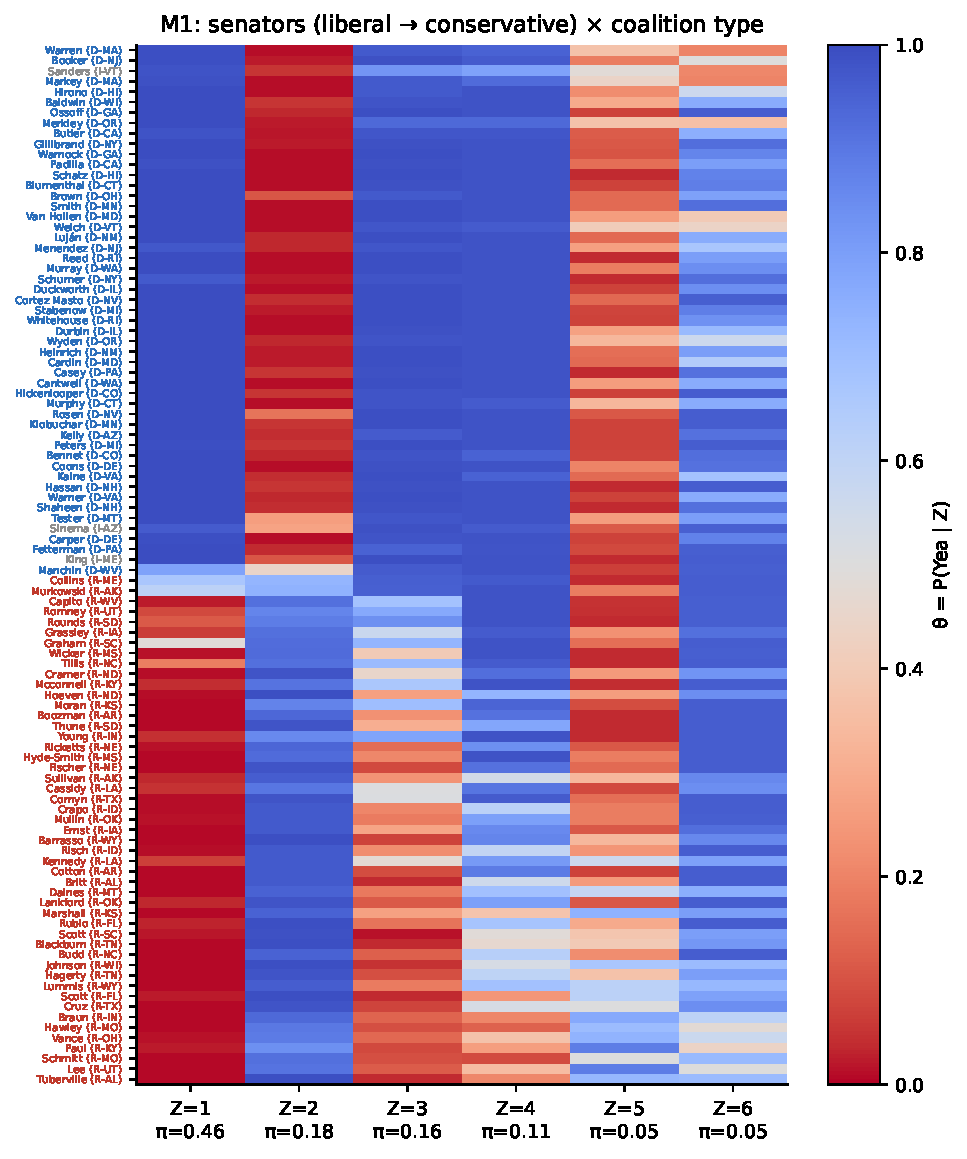
\includegraphics[width=\linewidth]{m1_theta_heatmap.pdf}\\[-2pt]{\small (a)}
\end{minipage}\hfill
\begin{minipage}[c]{0.54\linewidth}\centering
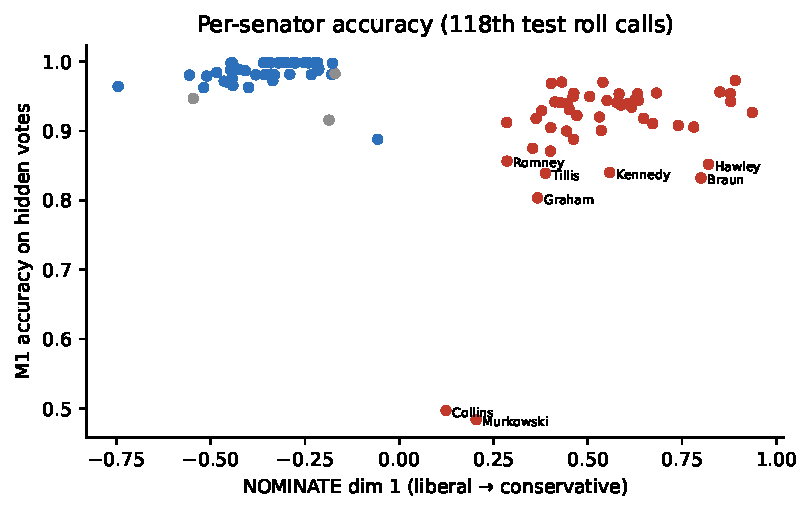
\includegraphics[width=\linewidth]{E3_per_senator.pdf}\\[-2pt]{\small (b)}
\end{minipage}
\vspace{2pt}
\caption{(a) M1 parameters $\theta_{iz}=P(\text{Yea}\mid Z{=}z)$: senators sorted liberal $\to$ conservative,
vote types sorted by frequency $\pi$. (b) M1 accuracy per senator on hidden test votes; the least predictable
senators are labeled.}
\label{fig:m1}
\end{figure}

\subsection{What the models reveal about the Senate}
None of these findings used party or state labels during training; the labels were only used to read the results.
\begin{itemize}
\item \textbf{A few vote types describe most roll calls} (Fig.~\ref{fig:m1}a). The largest type (46\% of roll calls)
is a Democratic-backed party-line vote; 229 of its 243 training roll calls are nominations or cloture motions, i.e.\
confirmation fights. The mirror image (18\%) is Republican-backed, mostly amendments and resolutions of disapproval.
Two bipartisan types are opposed only by shrinking conservative wings, and two small ``fringe'' types capture a
populist/libertarian right voting Yea alone and progressive Democrats voting Nay alone.
\item \textbf{Bridges between the parties are rare.} Only 6 of the 99 tree edges cross party lines (Fig.~\ref{fig:graphs}).
\item \textbf{Home-state pairs vote together.} 6 of the 10 strongest Ising couplings join the two senators of one
state (Crapo--Risch $W=1.99$, Reed--Whitehouse, Boozman--Cotton, Cantwell--Murray, Heinrich--Luj\'an,
Cramer--Hoeven).
\item \textbf{The swing senators are the hard cases.} Collins and Murkowski are the least predictable senators
(Fig.~\ref{fig:m1}b; M1 is right only half the time). They are tightly coupled to each other ($W=0.87$, the strongest
cross-ideology pair), which is why M3 does better on them. Graham is next (0.80).
\item \textbf{The left flank is the blind spot.} The hardest test roll call was the 17--79 vote of Nov.~20, 2024 on
blocking an arms-export license to Israel: 15 Democrats and 2 Independents voted Yea, no Republicans did. M1 has no
``progressive-only'' vote type, because such revolts are rare, so it treated the vote as a right-fringe revolt and
got 68\% of it right.
\item \textbf{Senators' positions are stable; the agenda changes.} Refitting only how often each vote type occurs
recovers almost all of the transfer gap (E4). For the Senate seated in January 2027, models of returning senators
are usable from day one; only newcomers need new data.
\end{itemize}

\begin{figure}[t]
\centering
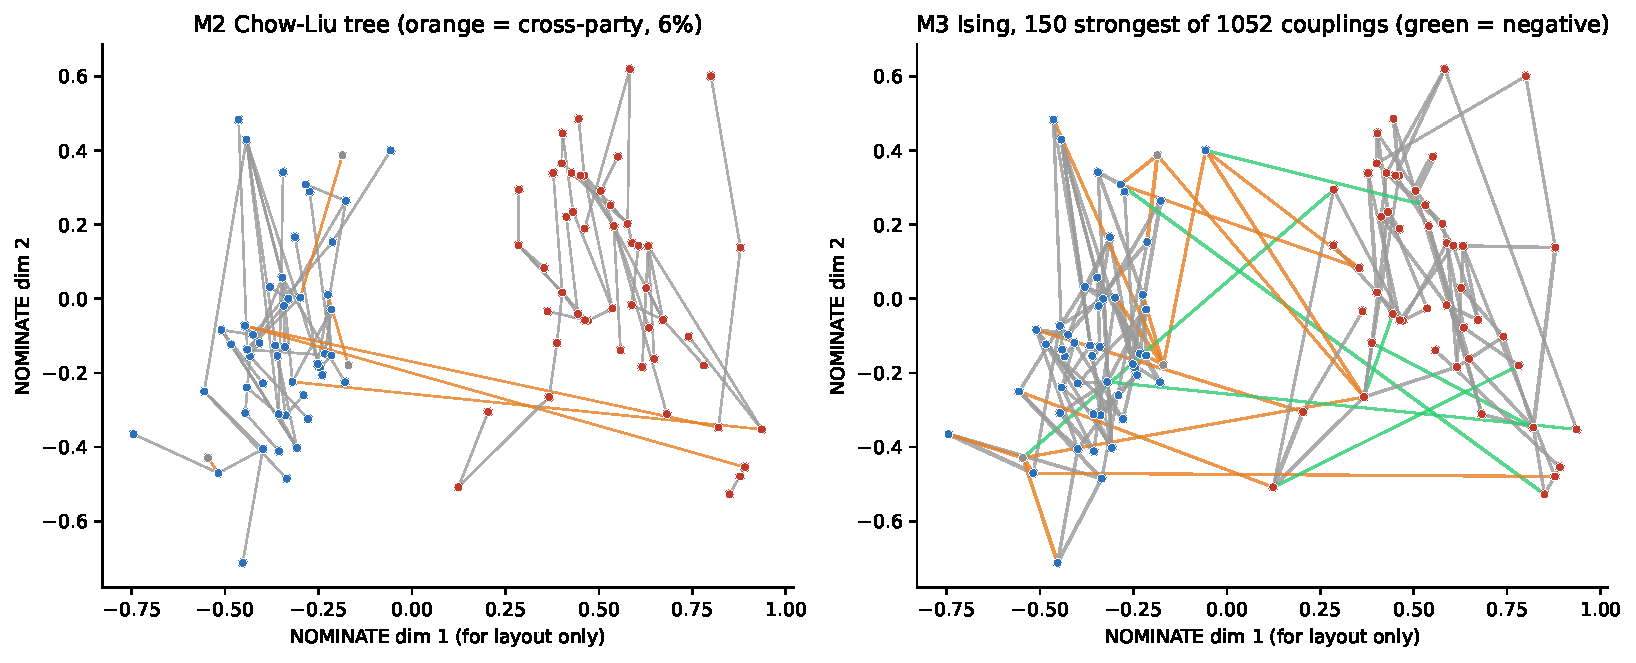
\includegraphics[width=0.82\linewidth]{graphs_tree_ising.pdf}
\vspace{-6pt}
\caption{Learned graphs on the 118th Senate, drawn at senators' NOMINATE coordinates (layout only). Blue/red nodes
= D/R. Left: Chow-Liu tree. Right: the 150 strongest Ising couplings; orange = cross-party, green = negative.}
\label{fig:graphs}
\end{figure}


\section{Conclusion and Limitations}
\subsection{Conclusion}
Of the three models, the simplest, a latent class with six vote types, is the best default: it gives the
best-calibrated predictions, its vote types are easy to read, it handles missing votes cleanly through EM, and it
carries over to a new Senate almost without loss. The Chow-Liu tree offers cheap exact inference but links the
parties through only a few edges. The sparse Ising model finds specific alliances, such as home-state pairs and
Collins--Murkowski, and matches the others' accuracy once its sparsity is tuned to the task, but it is less well
calibrated and needs approximate inference. Methodologically, mean-field is fast but overconfident under strong
coupling, missing votes should be marginalized rather than imputed, and hyper-parameters should be chosen with the
score of the reported task. Politically, Senate voting is dominated by party-line confirmation fights plus a few
recurring patterns; senators' positions persist across Congresses, and the hard votes come from a few swing senators
and rare revolts on either flank.

\subsection{Limitations}
We assume votes are missing at random, although absences can be strategic, and we treat roll calls as independent,
ignoring their order and content. Only 20 test roll calls are cross-cutting, so conclusions about them are noisy, and
E1 uses a single 16-senator model. Natural extensions are a latent class plus sparse residual couplings, an HMM over
roll calls to model the agenda, and bill content as an observed parent of $Z$.

\section{Reflections \& Contributions}
\textbf{Iteration.} Several decisions changed during the project:
\begin{itemize}
\item Our proposal treated $Z$ as a senator's party; since each sample is a roll call, we redefined $Z$ as the vote type.
\item Model selection first used the test split; we added a separate validation split.
\item $K$ and $\lambda$ first landed on the edges of their grids; we widened the grids.
\item M3's $\lambda$ was first chosen by pseudo-likelihood. Diagnosing weak 117th results showed this criterion, not
Gibbs mixing, was the cause; choosing $\lambda$ by the prediction task raised accuracy from 0.912 to 0.930.
\item Brute-force checks caught a bug in our own test harness, and a misleading convergence plot was replaced.
\item Stochastic EM for M3 brought little gain; we report it as a negative result.
\end{itemize}

\textbf{Advice for future students.} Verify every inference routine against brute force on tiny models before using
real data. Write down what one sample is before choosing latent variables. Keep the test split untouched until the
end, and choose hyper-parameters with the score of the task you report.

\textbf{Individual contributions and reflections.} \todo{Each member writes 1--2 sentences on their specific
tasks and a brief personal reflection, e.g.:}
\begin{itemize}
\item \todo{Name 1}: \todo{contribution}. \todo{reflection}.
\item \todo{Name 2}: \todo{contribution}. \todo{reflection}.
\item \todo{Name 3}: \todo{contribution}. \todo{reflection}.
\item \todo{Name 4}: \todo{contribution}. \todo{reflection}.
\item \todo{Name 5}: \todo{contribution}. \todo{reflection}.
\end{itemize}

\textbf{Use of generative AI.} We used Claude (Anthropic) to review the proposal against the course requirements,
to draft the notebook implementation, and to draft this report. \todo{Team: describe how you reviewed, tested and
adapted the AI-generated code and text, and which parts you wrote yourselves.}

\phantomsection\label{endmain}
\begin{thebibliography}{99}\small
\setlength{\itemsep}{1pt}
\bibitem{banerjee2008} O.~Banerjee, L.~El~Ghaoui, and A.~d'Aspremont. Model selection through sparse maximum
likelihood estimation for multivariate Gaussian or binary data. \emph{JMLR}, 9:485--516, 2008.
\bibitem{beck2009} A.~Beck and M.~Teboulle. A fast iterative shrinkage-thresholding algorithm for linear inverse
problems. \emph{SIAM J.\ Imaging Sciences}, 2(1):183--202, 2009.
\bibitem{besag1975} J.~Besag. Statistical analysis of non-lattice data. \emph{The Statistician}, 24(3):179--195, 1975.
\bibitem{chowliu1968} C.~Chow and C.~Liu. Approximating discrete probability distributions with dependence trees.
\emph{IEEE Trans.\ Information Theory}, 14(3):462--467, 1968.
\bibitem{clinton2004} J.~Clinton, S.~Jackman, and D.~Rivers. The statistical analysis of roll call data.
\emph{American Political Science Review}, 98(2):355--370, 2004.
\bibitem{dempster1977} A.~P.~Dempster, N.~M.~Laird, and D.~B.~Rubin. Maximum likelihood from incomplete data via the
EM algorithm. \emph{J.\ Royal Statistical Society B}, 39(1):1--38, 1977.
\bibitem{geman1984} S.~Geman and D.~Geman. Stochastic relaxation, Gibbs distributions, and the Bayesian restoration of
images. \emph{IEEE TPAMI}, 6(6):721--741, 1984.
\bibitem{voteview} J.~B.~Lewis, K.~Poole, H.~Rosenthal, A.~Boche, A.~Rudkin, and L.~Sonnet. Voteview: Congressional
roll-call votes database. \url{https://voteview.com/}, accessed Oct.\ 2026.
\bibitem{poole1985} K.~T.~Poole and H.~Rosenthal. A spatial model for legislative roll call analysis.
\emph{American Journal of Political Science}, 29(2):357--384, 1985.
\bibitem{ravikumar2010} P.~Ravikumar, M.~J.~Wainwright, and J.~D.~Lafferty. High-dimensional Ising model selection
using $\ell_1$-regularized logistic regression. \emph{Annals of Statistics}, 38(3):1287--1319, 2010.
\bibitem{rubin1976} D.~B.~Rubin. Inference and missing data. \emph{Biometrika}, 63(3):581--592, 1976.
\bibitem{wainwright2008} M.~J.~Wainwright and M.~I.~Jordan. Graphical models, exponential families, and variational
inference. \emph{Foundations and Trends in Machine Learning}, 1(1--2):1--305, 2008.
\end{thebibliography}

\appendix
\section{Algorithm Details}\label{app:alg}
\textbf{M1: EM updates.} With $Y_{mi}=[x_{mi}{=}{+}1]$, $N_{mi}=[x_{mi}{=}{-}1]$ and $O_m$ the senators observed on
roll call $m$:
\begin{align*}
\text{E-step:}\quad &\gamma_{mk}\propto\pi_k\prod_{i\in O_m}\theta_{ik}^{Y_{mi}}(1-\theta_{ik})^{N_{mi}},\\
\text{M-step:}\quad &\pi_k=\frac{\sum_m\gamma_{mk}+c_k}{M+\sum_{k'}c_{k'}},\qquad
\theta_{ik}=\frac{\sum_m\gamma_{mk}Y_{mi}+a_{ik}}{\sum_m\gamma_{mk}(Y_{mi}+N_{mi})+a_{ik}+b_{ik}}.
\end{align*}
These are MAP updates under Beta($a{+}1,b{+}1$) and Dirichlet($c{+}1$) priors. We use $a=b=c=1$ by default. In E4,
$a=s\,\theta^{(117)}$, $b=s(1-\theta^{(117)})$ and $c=s\,\pi^{(117)}$ turn the 117th-Senate fit into a prior of
strength $s$.

\textbf{M2: belief propagation.} Let $\lambda_i(x_i)$ be the evidence indicator: one-hot if senator $i$'s vote is
observed, all ones otherwise. The upward pass (leaves first) computes
$\beta_i(x_i)=\lambda_i(x_i)\prod_{c\in\mathrm{ch}(i)}m_{c\to i}(x_i)$ and
$m_{i\to p}(x_p)=\sum_{x_i}P(x_i\mid x_p)\,\beta_i(x_i)$, normalizing each $\beta_i$; the log normalizers sum to
$\log P(\mathbf x_O)$. The downward pass computes
$\alpha_i(x_i)\propto\sum_{x_p}P(x_i\mid x_p)\,\alpha_p(x_p)\beta_p(x_p)/m_{i\to p}(x_p)$ from the root prior. Node
marginals are $\propto\alpha_i\beta_i$, and the (parent, child) pair marginals that EM needs are
$\propto[\alpha_p\beta_p/m_{i\to p}](x_p)\,P(x_i\mid x_p)\,\beta_i(x_i)$.

\textbf{M3: pseudo-likelihood and FISTA.} With local field $h_{mi}=\theta_i+\sum_jW_{ij}x_{mj}$ we minimize
\[
F(\theta,W)=\frac1M\sum_m\sum_{i\in O_m}\log\big(1+e^{-2x_{mi}h_{mi}}\big)+\lambda\sum_{i<j}|W_{ij}|.
\]
Writing $r_{mi}=2x_{mi}\,\sigma(-2x_{mi}h_{mi})$ for observed entries, the gradient of the smooth part is
$-\frac1M\sum_m r_{mi}$ for $\theta_i$ and $-\frac1M\sum_m(r_{mi}x_{mj}+r_{mj}x_{mi})$ for the shared coupling
$W_{ij}$. Each FISTA step is a gradient step followed by soft-thresholding of $W$ at $\lambda/L$, with $L$ found by
backtracking. $\lambda$ is chosen by NLL on the 20\%-reveal task on the validation split.

\textbf{M3: inference.} Gibbs resamples each unobserved $x_i$ from $\sigma(2h_i)$ and estimates marginals by
averaging these conditional probabilities after burn-in (Rao-Blackwellization), which has lower variance than
averaging 0/1 samples. Mean-field updates $\mu_i$ one at a time; each update minimizes the variational free energy
in $\mu_i$, so the sweep converges.

\section{Additional Figures and Tables}

\begin{table}[h]
\centering\small
\caption{Correctness checks against brute-force enumeration (random 6-variable models) and synthetic recovery.}
\label{tab:checks}
\begin{tabular}{lr}
\toprule
Check & Error\\
\midrule
M1 exact inference vs.\ brute force (max abs, unobserved votes) & $<10^{-14}$\\
M2 BP marginals / $\log P(\mathbf x_O)$ vs.\ brute force (max abs) & $<10^{-14}$\\
Ising exact enumeration vs.\ brute force (max abs) & $<10^{-14}$\\
Ising Gibbs, 3000 sweeps (mean abs) & $1.4\times10^{-3}$\\
M1 EM, 30\% missing, 3000 samples: max $|\hat\theta-\theta|$ & 0.050\\
Chow-Liu edge recovery, 30-node tree, 3000 samples & 26/29\\
\bottomrule
\end{tabular}
\end{table}

\begin{table}[h]
\centering\small
\caption{Diagnosing M3 on the E3 task (3 reveals): more Gibbs sweeps vs.\ the pseudo-likelihood choice of $\lambda$.}
\label{tab:diag}
\begin{tabular}{lcccc}
\toprule
& \multicolumn{2}{c}{117th} & \multicolumn{2}{c}{118th}\\
\cmidrule(lr){2-3}\cmidrule(lr){4-5}
M3 variant & Acc & NLL & Acc & NLL\\
\midrule
Task-selected $\lambda$ (0.01 / 0.02), Gibbs 300 sweeps & 0.930 & 0.186 & 0.949 & 0.148\\
Task-selected $\lambda$, Gibbs 3000 sweeps & 0.932 & 0.190 & 0.948 & 0.150\\
Pseudo-likelihood $\lambda=0.05$, Gibbs 300 sweeps & 0.912 & 0.233 & 0.943 & 0.154\\
Pseudo-likelihood $\lambda=0.05$, mean-field & 0.886 & 0.339 & 0.935 & 0.201\\
\bottomrule
\end{tabular}
\end{table}

\begin{table}[h]
\centering\small
\caption{Vote questions of 118th training roll calls by most likely M1 coalition type.}
\begin{tabular}{lrrrrrr}
\toprule
Vote question & $Z_1$ & $Z_2$ & $Z_3$ & $Z_4$ & $Z_5$ & $Z_6$\\
\midrule
On the Nomination & 114 & 0 & 36 & 20 & 0 & 1\\
On the Cloture Motion & 115 & 0 & 35 & 19 & 0 & 4\\
On the Amendment & 1 & 40 & 3 & 3 & 17 & 4\\
On the Joint Resolution & 0 & 19 & 0 & 0 & 0 & 2\\
On the Motion / to Table & 5 & 20 & 1 & 4 & 5 & 3\\
Other & 8 & 15 & 11 & 10 & 3 & 9\\
\bottomrule
\end{tabular}
\end{table}

\begin{figure}[h]
\centering
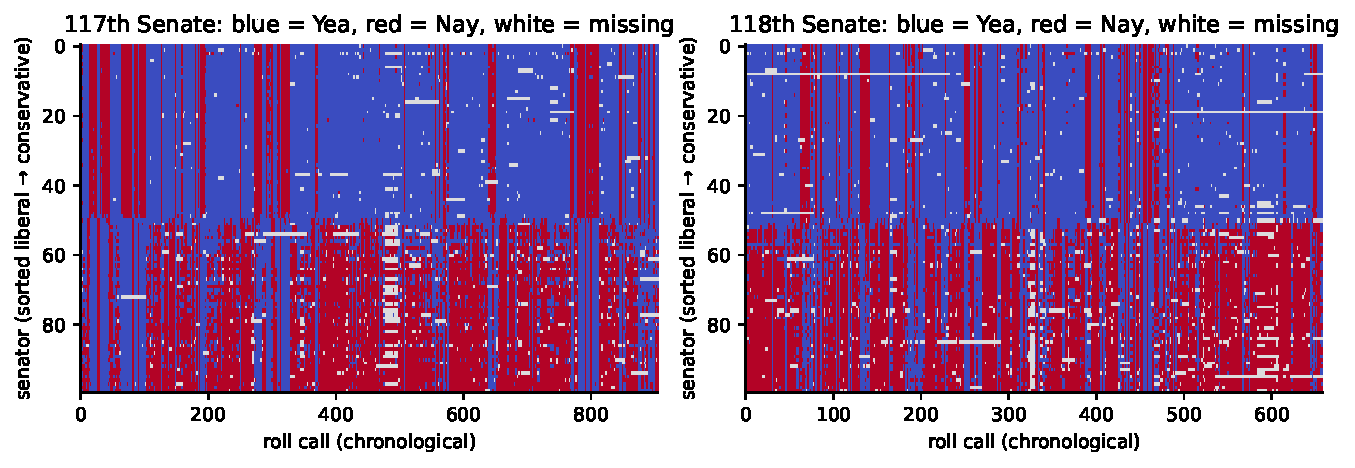
\includegraphics[width=0.95\linewidth]{data_vote_matrix.pdf}
\caption{Vote matrices after preprocessing (senators sorted by NOMINATE dimension 1).}
\end{figure}

\begin{figure}[h]
\centering
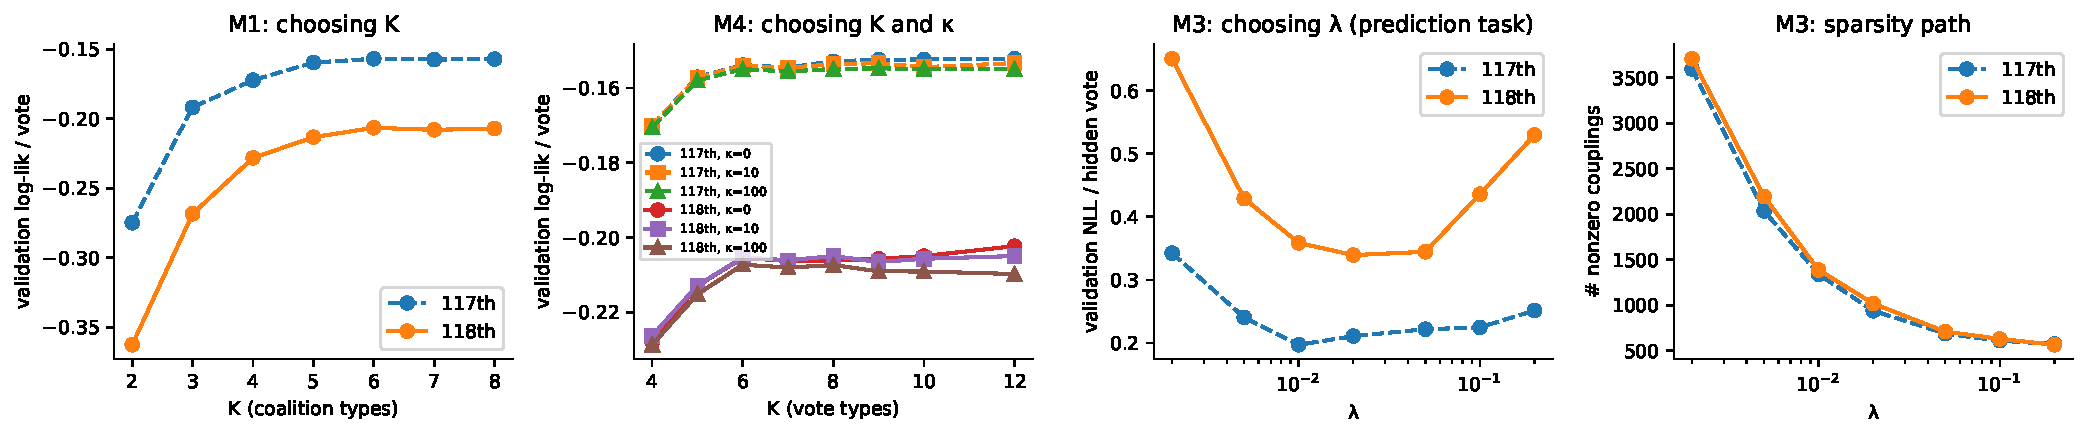
\includegraphics[width=\linewidth]{model_selection.pdf}
\caption{Model selection on the validation split: M1's $K$ (log-likelihood), M3's $\lambda$ (NLL on the 20\%-reveal
prediction task), and M3's number of couplings.}
\label{fig:selection}
\end{figure}

\begin{figure}[h]
\centering
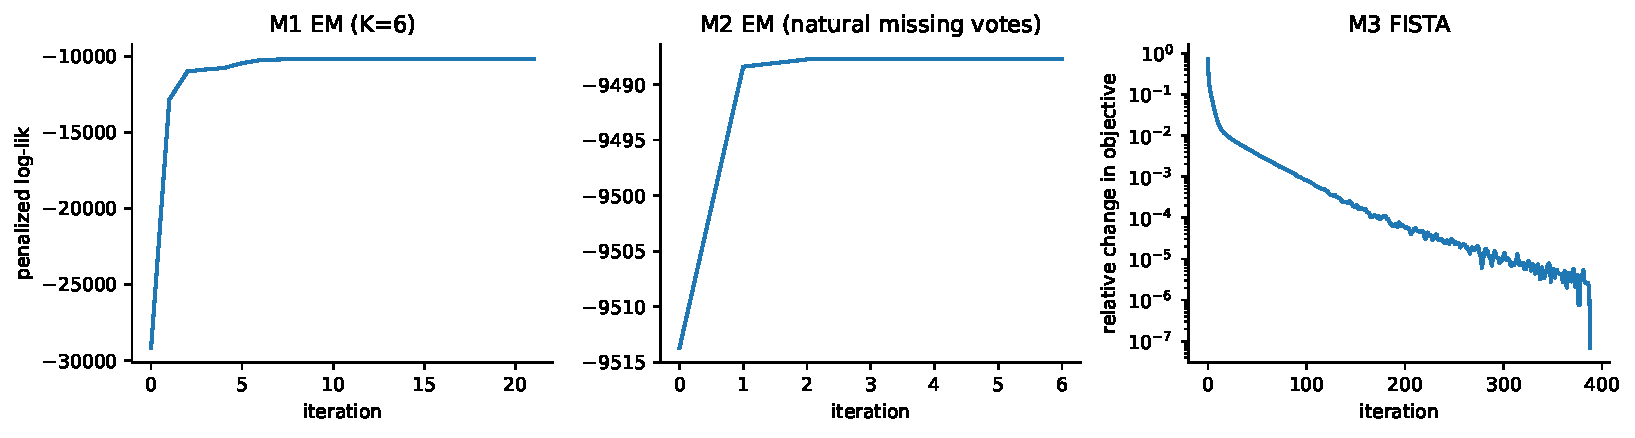
\includegraphics[width=\linewidth]{convergence.pdf}
\caption{Convergence on the 118th training data: M1 EM, M2 EM (penalized log-likelihood), and the relative change
of the M3 FISTA objective per iteration.}
\label{fig:conv}
\end{figure}

\begin{figure}[h]
\centering
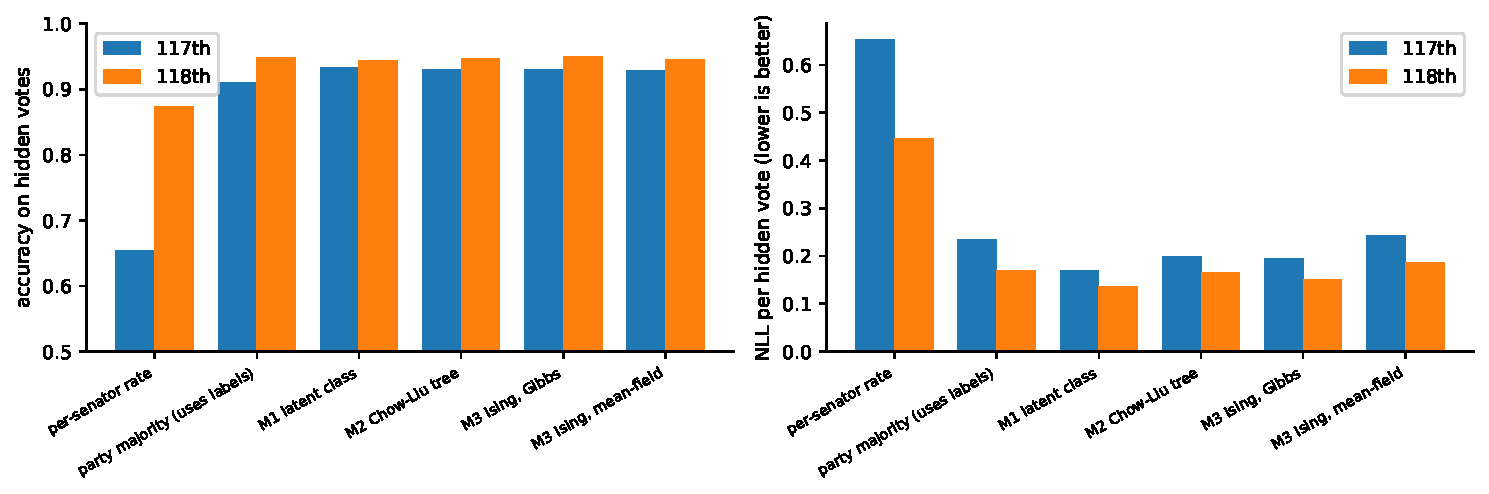
\includegraphics[width=0.9\linewidth]{E3_comparison.pdf}
\caption{E3 accuracy and NLL for both Congresses.}
\end{figure}

\end{document}
